\documentclass{article}
\usepackage[utf8]{inputenc}
\usepackage{amssymb}
\usepackage{amsmath}
\usepackage{float}
\usepackage{epstopdf}
\usepackage{moreverb}
\usepackage{multicol}
\usepackage{listings}
\usepackage{mathrsfs}
\usepackage{graphicx}
\usepackage{cite}
\usepackage{tabularx}
\usepackage{listings}
\usepackage{subcaption}
\newcommand{\R}{\mathbb{R}}
\newcommand{\overbar}[1]{\mkern 1.5mu\overline{\mkern-1.5mu#1\mkern-1.5mu}\mkern 1.5mu}
\newcommand{\pdiff}[2]{\frac{\partial {#1}}{\partial {#2}}}


\bibliographystyle{plain}
\title{APPM 5720 Homework 5}
\author{Wil Boshell, Fortino Garcia, Alex Rybchuk, Parth Thakkar}
\date{February 22, 2018}


\begin{document}

\maketitle

\maketitle

\noindent The main task of this homework is to approximate the transport equation
	\begin{align*}
		u_t + \left( a u\right)_x = 0, \quad x_L \leq x \leq x_R, \quad t > 0,
	\end{align*}
with initial conditions $u(x,0) = f(x)$.

\section{Mapping with Straight-Sided Quadrilaterals}
In order to move from one-dimensional DG methods to two-dimensional DG methods, a mapping between the domain of the geometry and the reference domain $[-1,1]^2$ is required. One way to achieve this is with a simple bilinear mapping,

\begin{equation}
X(r,s) = \alpha_1 + \alpha_2r + \alpha_3s + \alpha_4rs, \\
Y(r,s) = \beta_1 + \beta_2r + \beta_3s + \beta_4rs
\end{equation} 

The value of the coefficients $\alpha_i$, $\beta_i$ can be found by evaluating $X(r,s)$ in each of the corners of the reference domain

\begin{equation}
    \begin{bmatrix}
      x_1 \\
      x_2 \\
      x_3 \\
      x_4 
    \end{bmatrix}
    =     
    \begin{bmatrix}
      1 & -1 & -1 & 1 \\
      1 & 1 & -1 & -1 \\
      1 & 1 & 1 & 1 \\
      1 & -1 & 1 & -1
    \end{bmatrix}
    \begin{bmatrix}
      \alpha_1 \\
      \alpha_2 \\
      \alpha_3 \\
      \alpha_4 
    \end{bmatrix}.
\end{equation}

This mapping is demonstrated below.

\begin{figure}[H]
  \centering
  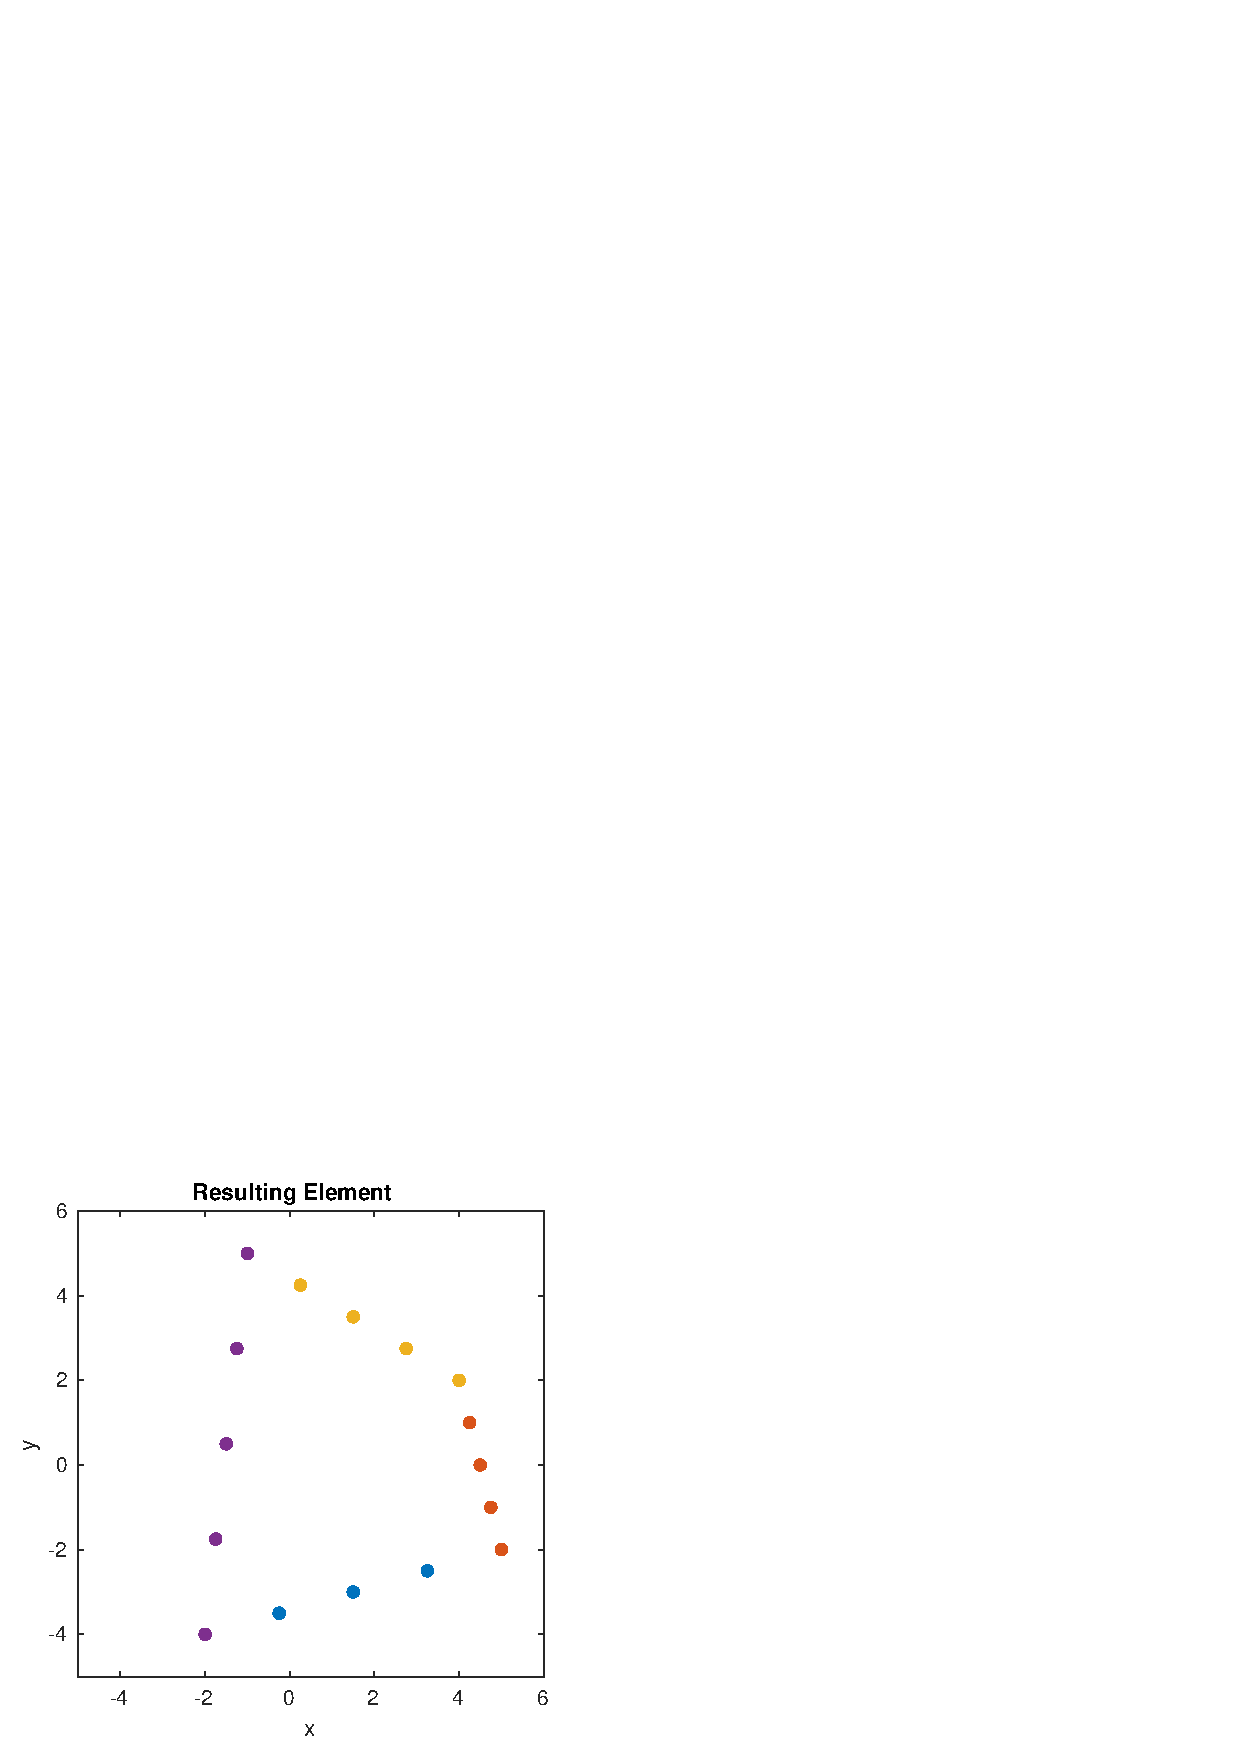
\includegraphics[scale=0.5]{media/5-1-xy.png}
  \includegraphics[scale=0.5]{media/5-1-rs.png}
  
  \caption{Mapping from the element domain to the reference domain $[-1,1]^2$.}
  \label{fig:spatDer}
\end{figure}

\noindent With this mapping, integrals of functions in the $(x,y)$ domain can be computed through a change of variables

\begin{equation}
\int \int f(x,y) dx dy = \int \int f(x(r,s), y(r,s)) |J| dr ds,
\end{equation} 

where

\begin{equation*}
|J| =    \lvert \begin{bmatrix}
      \frac{dx}{dr} & \frac{dx}{ds}\\
      \frac{dy}{dr} & \frac{dy}{ds}
    \end{bmatrix} \rvert
\end{equation*}

In order to verify this mapping, the area of a perturbed grid with straight-sided edges was calculated. 

The value of area was found to be independent of the grid resolution as well as the degree of quadrature. This behavior is expected because here the element domain maps exactly to the reference domain.

\begin{figure}[H]
  \centering
  \includegraphics[scale=0.5]{media/5-2-rs.png}
  
  \caption{Mapping from the element domain to the reference domain $[-1,1]^2$.}
  \label{fig:spatDer}
\end{figure}

A similar area calculation was carried out for elements with curvilinear sides. Here the area was not calculated exactly because the element domain does not exactly map to the reference domain. The error was seen to follow $min(n_r,n_s)$, where $(n_r, n_s)$ are the number of discretization points.

\begin{figure}[H]
  \centering
  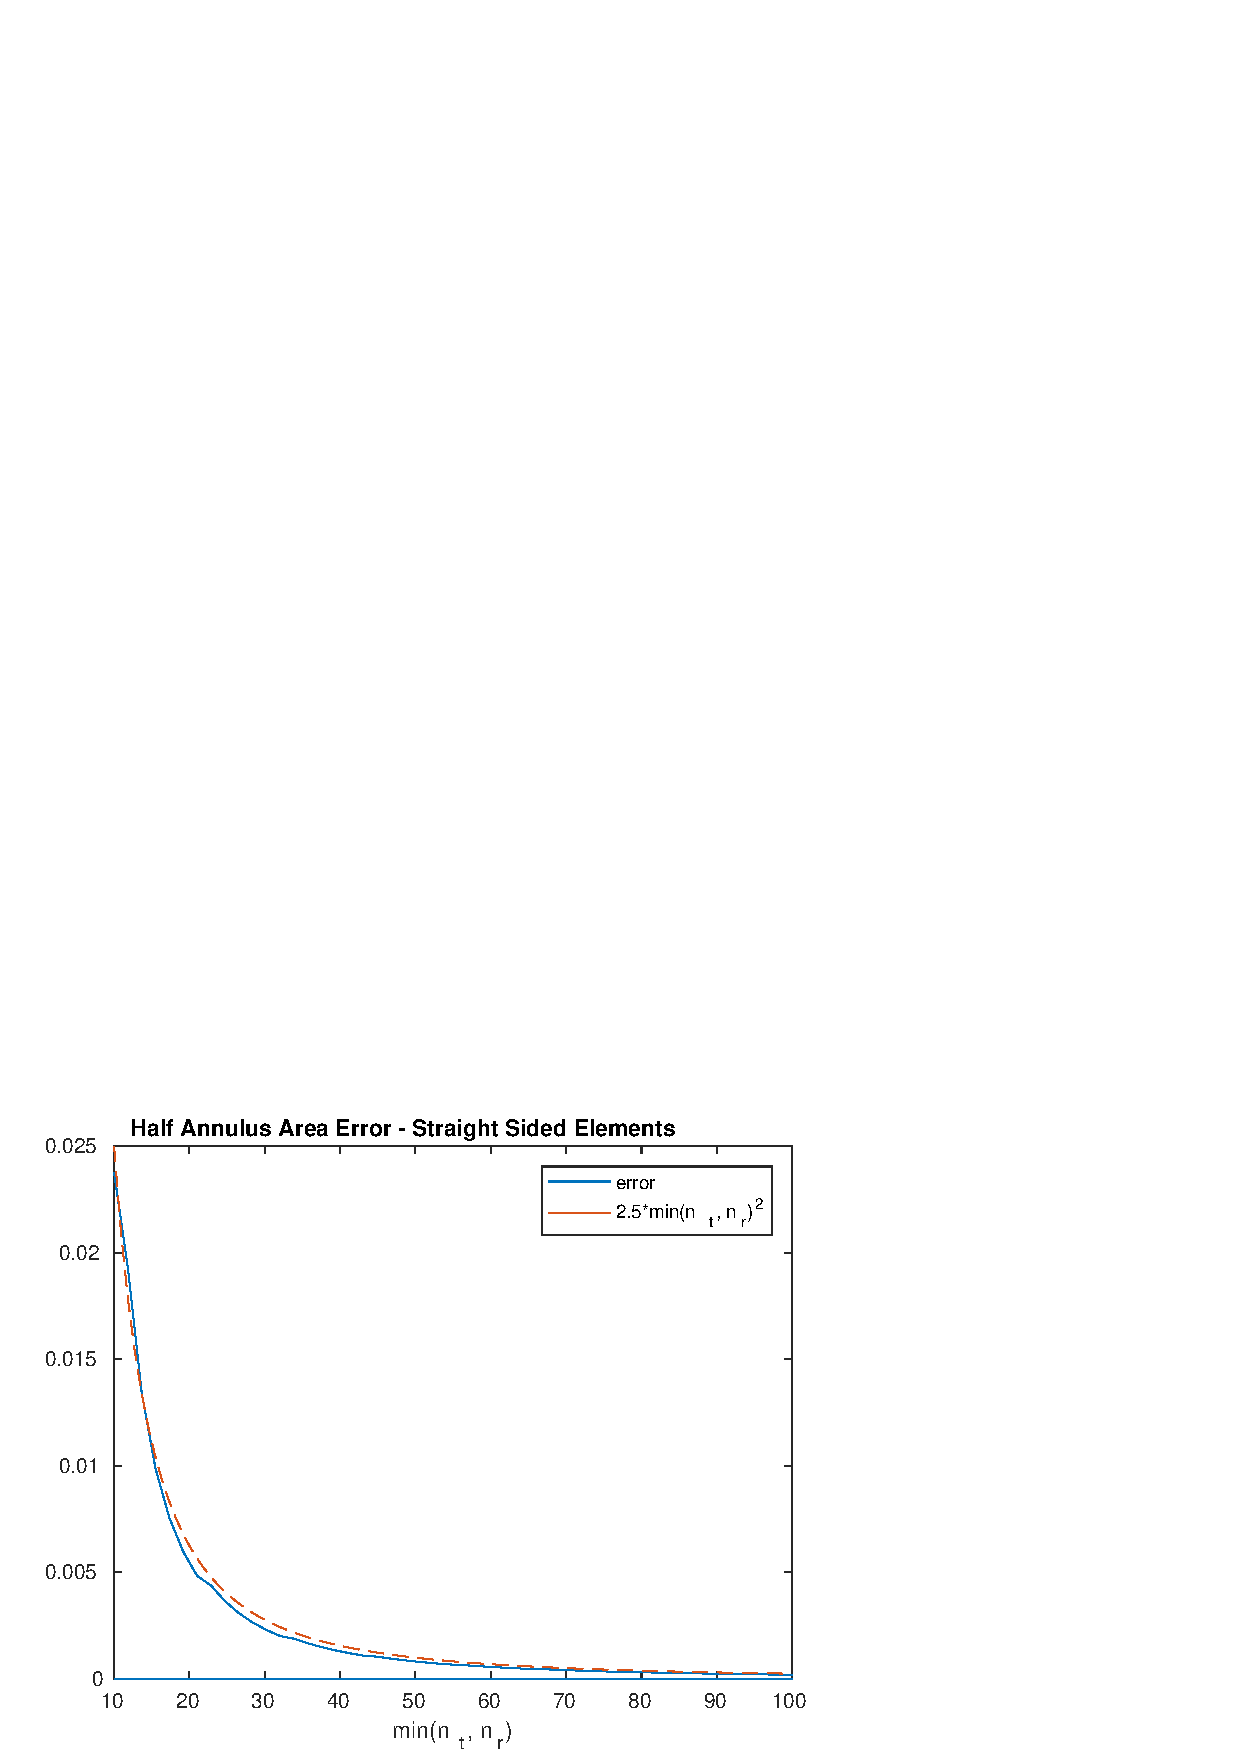
\includegraphics[scale=0.5]{media/5-3-error.png}
  
  \caption{Error on area for curilinear elements.}
  \label{fig:spatDer}
\end{figure}

\noindent As before, we notice that we get steadily decreasing error until we achieve aroun $11-12$ digits of accuracy, after which roundoff errors steadily increase the error in the computation of the derivative. To further understand this process, we compute the eigenvalues of the matrix $A$, defined through $\boldsymbol{\hat{b}} = A \boldsymbol{\hat{u}}$. We assume periodic boundary conditions and a constant coefficient $a = 1$ for the following plots, which were generated by calling \verb|dgeev| and ploting via MATLAB. First let us examine the behavior of $\lambda _{max}$ with respect to increasing $q$ (and here we normalize by the scaling factor in the affine map):


\section{Mapping with Curvi-Linear Quadrilaterals}


\subsection{Gordon-Hall Mapping}
\noindent In order to use the mapping to compute integrals (and derivatives) we will need to compute the metric, i.e. $r_x, \, r_y, \, s_x, \, s_y$. Recall that the chain rule for a function of two variables requires that:
  \begin{align*}
    \pdiff{u(x(r,s),y(r,s))}{x} & = \pdiff{r}{x}\pdiff{u}{r} + \pdiff{s}{x} \pdiff{u}{s}, \\
    \pdiff{u(x(r,s),y(r,s))}{y} & = \pdiff{r}{y}\pdiff{u}{r} + \pdiff{s}{y} \pdiff{u}{s}.
  \end{align*}
By substituting $u = x$ and $u = y$ into the above equations, we arrive at:
  \begin{align*}
    1 & = \pdiff{x}{x} = \pdiff{r}{x}\pdiff{x}{r} + \pdiff{s}{x} \pdiff{x}{s} = r_x x_r + s_x x_s, \\
    1 & = \pdiff{y}{y}  = \pdiff{r}{y}\pdiff{y}{r} + \pdiff{s}{y} \pdiff{y}{s} = r_y y_r + s_y y_s.  
  \end{align*}
Rewriting this as a matrix system, we arrive at 

  \begin{equation}
    \begin{bmatrix}
      1 & 0 \\
      0 & 1
    \end{bmatrix}
    = 
    \begin{bmatrix}
      r_x & s_x \\
      r_y & s_y
    \end{bmatrix}
    \begin{bmatrix}
      x_r & y_r \\
      x_s & y_s
    \end{bmatrix}.
  \end{equation}
Using the explicit formula for the inverse of a matrix, we immediately solve for the metric via
  \begin{equation}
    \begin{bmatrix}
      r_x & s_x \\
      r_y & s_y
    \end{bmatrix}
    =
    \begin{bmatrix}
      x_r & y_r \\
      x_s & y_s
    \end{bmatrix}^{-1}
    = \frac{1}{x_r y_s - x_s y_r}
    \begin{bmatrix}
      y_s & -y_r \\
      -x_s & x_r
    \end{bmatrix}
    = \frac{1}{J}
    \begin{bmatrix}
      y_s & -y_r \\
      -x_s & x_r
    \end{bmatrix}.
  \end{equation}
where $J = x_r y_s - x_s y_r$. Note that this gives

\subsection{Line Integrals}
We now consider finding the area of an element via line integrals (instead of the previously direct volume integral). To that end, consider the vector field $F(x,y) = (x/2, y/2)$. Then $\nabla \cdot F(x,y) = 1$ and by the divergence theorem:

  \begin{align*}
    V =  \int_\Omega 1 \, dV = \int_\Omega \nabla \cdot F(x,y) \, dV = \int_{\partial \Omega} \nabla F(x,y) \cdot \hat{\textbf{n}} \, dl = \int_{\partial \Omega} \left( \frac{x}{2}n_1 + \frac{y}{2}n_2 \right)\, dl,
  \end{align*}
where $\hat{\textbf{n}} = (n_1,n_2)$. If we consider the reference square, side 1 corresponds to $s = 1$ and $r \in [-1,1]$. The tangent to the curve along this face is clearly $(x_r,y_r)$ so that the normal is
  \begin{align*}
    (-y_r, \, x_r) = J (s_x, \, s_y) \implies \hat{\boldsymbol{n_1}} = \frac{(s_x, \, s_y)}{\sqrt{s_x^2 + s_y^2}}.
  \end{align*}
A similar calculation for the other 3 faces will yield the following set of normals (where the subscript indicates which face it belongs to):

  \begin{align*}
    \hat{\boldsymbol{n_1}} = \frac{(s_x, \, s_y)}{\sqrt{s_x^2 + s_y^2}}, & \quad
    \hat{\boldsymbol{n_2}} = -\frac{(r_x, \, r_y)}{\sqrt{r_x^2 + r_y^2}}, \\
    \hat{\boldsymbol{n_3}} = -\frac{(s_x, \, s_y)}{\sqrt{s_x^2 + s_y^2}}, & \quad
    \hat{\boldsymbol{n_4}} = \frac{(r_x, \, r_y)}{\sqrt{s_x^2 + s_y^2}}. \\
  \end{align*}

% \begin{figure}[H]
%   \centering
%   \includegraphics[scale=0.7]{plots/eig_data.png}
%   \caption{Plot of $\lambda _{max}$ with Increasing $q$}
%   \label{fig:eig_data}
% \end{figure}

% \begin{figure}[H]
%   \centering
%   \begin{minipage}{.4\textwidth}
%     \centering
%     \includegraphics[width=\linewidth]{plots/l2_time_1.png}
%     \label{fig:smallstep}
%   \end{minipage}%
%   \begin{minipage}{.4\textwidth}
%     \centering
%     \includegraphics[width=\linewidth]{plots/l2_time_2.png}
%     \label{fig:medstep}
%   \end{minipage}%
%   \begin{minipage}{.4\textwidth}
%     \centering
%     \includegraphics[width=\linewidth]{plots/l2_time_3.png}
%     \label{fig:bigstep}
%   \end{minipage}%
% \end{figure}
\end{document}


